\documentclass[]{standalone}

% More defined colors
\usepackage[dvipsnames]{xcolor}

\usepackage{tikz}
\usetikzlibrary{positioning, petri, arrows.meta}

\tikzstyle{Func} = [rectangle, rounded corners, minimum width = 6mm, minimum height = 6mm, draw=blue!50, fill = blue!20]
\tikzstyle{Sum} = [circle, minimum width = 4mm, minimum height = 4mm, draw=black!50, fill = black!20, inner sep = 0cm, text = black]

\begin{document}

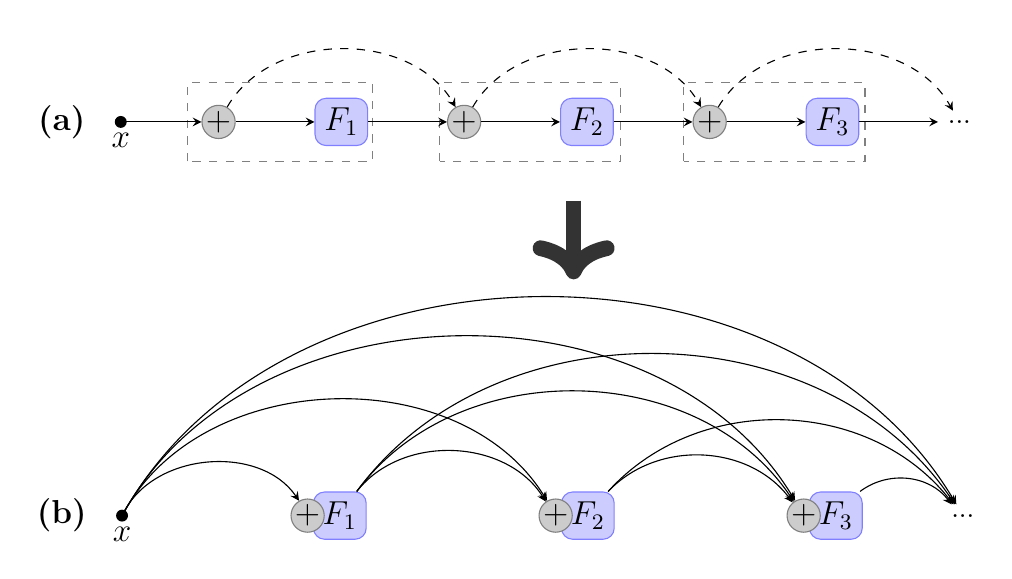
\begin{tikzpicture}

    %%%%%%%%%%%%%%%%%%%%%%
    \node (title1) at (0,0) {\large\textbf{(a)}};
    \node [tokens=1, inner sep = 0mm, label=below:\large$x$] (start) [right=3mm of title1] {};

    \node[Sum] (sum1) [right=1cm of start] {\large +};
    \node[Func] (f1) [right=1cm of sum1] {\large $F_1$};
    \draw [black!50, dashed] (1.6, -0.5) rectangle (3.95, 0.5);

    \node[Sum] (sum2) [right=of f1] {\large +};
    \node[Func] (f2) [right=of sum2] {\large $F_2$};
    \draw [black!50, dashed] (4.8, -0.5) rectangle (7.1, 0.5);

    \node[Sum] (sum3) [right=of f2] {\large +};
    \node[Func] (f3) [right=of sum3] {\large $F_3$};
    \draw [black!50, dashed] (7.9, -0.5) rectangle (10.2, 0.5);

    \node (end) [right=of f3] {...};

    \draw[-stealth] (start) to (sum1);
    \draw[-stealth] (sum1) to (f1);
    \draw[-stealth] (f1) to (sum2);
    \draw[-stealth] (sum2) to (f2);
    \draw[-stealth] (f2) to (sum3);
    \draw[-stealth] (sum3) to (f3);  % , line width=1pt
    \draw[-stealth] (f3) to (end);
    \draw[-stealth, dashed] (sum1) to [bend left=60] (sum2);
    \draw[-stealth, dashed] (sum2) to [bend left=60] (sum3);
    \draw[-stealth, dashed] (sum3) to [bend left=60] (end);

    %%%%%%%%%%%%%%%%%%%%%%
    \node (title2) at (0,-5) {\large\textbf{(b)}};
    \node [tokens=1, inner sep = 0mm, label=below:\large$x$] (start) [right=3mm of title2] {};

    \node[Func] (f1) [right= 2.4cm of start] {\large $F_1$};
    \node[Sum] (sum1) [left=-1.5mm of f1] {\large +};

    \node[Func] (f2) [right= 3.0cm of sum1] {\large $F_2$};
    \node[Sum] (sum2) [left=-1.5mm of f2] {\large +};

    \node[Func] (f3) [right= 3.0cm of sum2] {\large $F_3$};
    \node[Sum] (sum3) [left=-1.5mm of f3] {\large +};

    \node[] (DAGend) [right=of f3] {...};

    \draw[-stealth] (start) to [bend left=60] (sum1);
    \draw[-stealth] (start) to [bend left=60] (sum2);
    \draw[-stealth] (start) to [bend left=60] (sum3);
    \draw[-stealth] (start) to [bend left=60] (DAGend);

    \draw[-stealth] (f1) to [bend left=55] (sum2);
    \draw[-stealth] (f1) to [bend left=55] (sum3);
    \draw[-stealth] (f1) to [bend left=55] (DAGend);

    \draw[-stealth] (f2) to [bend left=50] (sum3);
    \draw[-stealth] (f2) to [bend left=50] (DAGend);

    \draw[-stealth] (f3) to [bend left=45] (DAGend);

    %%%%%%%%%%%%%%%%%%%%%%%%%
    % \node[rectangle, rounded corners, text width=3.5cm, draw=black, fill=red!20] (NeuralNetwork) [right=3mm of end] {Architecture of residual neural networks};
    % \node[rectangle, rounded corners, text width=3.5cm, draw=black, fill=red!20] (DAG) [above right=4mm of DAGend] {Complete directed acyclic graph};
    \draw [arrows = {-Computer Modern Rightarrow[line join=round]}, line width=2mm, black!80] (6.5, -1) -- (6.5, -2);  %(NeuralNetwork) to (DAG);  % 

\end{tikzpicture}

\end{document}